\chapter{explore\_lite}

\section{Package Summary}

Lightweight frontier-based exploration.

\begin{itemize}
    \item Maintainer status: developed
    \item Maintainer: Jiri Horner \textless laeqten AT gmail DOT com\textgreater
    \item Author: Jiri Horner  \textless laeqten AT gmail DOT com\textgreater
    \item License: BSD
    \item Source: git \url{https://github.com/hrnr/m-explore.git} (branch: master)
\end{itemize}

\section{Overview}

This package provides greedy frontier-based exploration. When node is running, robot will greedily explore its enviroment until no frontiers could be found. Movement commands will be send to \href{http://wiki.ros.org/move_base}{move\_base}.

%{{attachment:screenshot.png||width="755px"}}

Unlike similar packages, \texttt{explore\_lite} does not create it's own costmap. Node subscribes to \texttt{nav\_msgs/OccupancyGrid} messages. Commands for robot movement are send to \href{http://wiki.ros.org/move_base}{move\_base} node.

\section{Architecture}

\texttt{explore\_lite} uses \href{http://wiki.ros.org/move_base}{move\_base} for navigation. You need to run properly configured \href{http://wiki.ros.org/move_base}{move\_base} node.

\begin{figure}
    \centering
    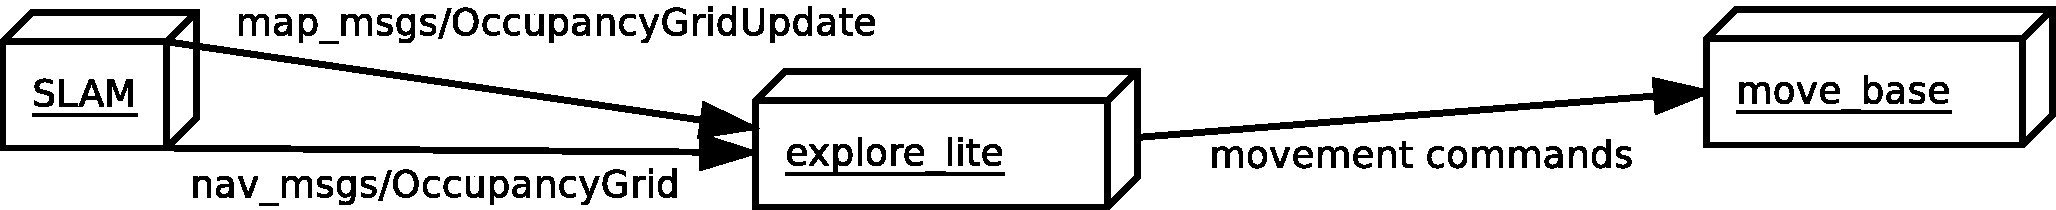
\includegraphics[width=\textwidth]{../img/explore_architecture.pdf}
    \caption{Architecture of \texttt{explore\_lite}, exploring node for \gls{ROS}.}
    \label{fig:mapmergearchitecture}
\end{figure}

\texttt{explore\_lite} subscribes to a \texttt{nav\_msgs/Occu\-pan\-cy\-Grid} and \texttt{map\_msgs/Occu\-pan\-cy\-Grid\-Up\-da\-te} messages to construct a map where it looks for frontiers. You can either use costmap published by \href{http://wiki.ros.org/move_base}{move\_base} (ie. \texttt{<mo\-ve\_ba\-se>/glo\-bal\_cost\-map/\-cost\-map}) or you can use map constructed by mapping algorithm (SLAM). Better results were achieved on maps constructed by SLAM as they usually contain less noise.

Currently \texttt{explore\_lite} also requires footprint information. Footprint is published by \href{http://wiki.ros.org/move_base}{move\_base} \texttt{move\_base/global\_costmap/footprint}. You can specify different footprint topic, but that should not be necassary. Default works for both circular and non-circular robots depending on \href{http://wiki.ros.org/move_base}{move\_base} configuration.

\section{ROS API}
\subsection{explore}

Provides exploration services offered by this package. Exploration will start immediately after node initialization.

\subsubsection{Actions Called}
  \ROStopic{move\_base}{move\_base\_msgs/MoveBaseAction}{\href{http://wiki.ros.org/move_base}{move\_base} actionlib API for posting goals. See \href{http://wiki.ros.org/move_base\#Action_API}{move\_base\#Action API} for details. This expects \href{http://wiki.ros.org/move_base}{move\_base} node in the same namespace as \texttt{explore\_lite}, you may want to remap this node if this is not true.}

\subsubsection{Subscribed Topics}
  \ROStopic{costmap}{nav\_msgs/OccupancyGrid}{Map which will be used for exploration planning. Can be either cost from \href{http://wiki.ros.org/move_base}{move\_base} or map created by SLAM (see above). Occupancy grid must have got properly marked unknown space, mapping algorithms usually track unknown space by default. If you want to use costmap provided by \href{http://wiki.ros.org/move_base}{move\_base} you need to enable unknown space tracking by setting \texttt{track\_unknown\_space: true}.}

  \ROStopic{costmap\_updates}{map\_msgs/OccupancyGridUpdate}{Incremental updates on costmap. Not necessary if source of map is always publishing full updates, i.e. does not provide this topic.}

  \ROStopic{footprint\_stamped}{geometry\_msgs/PolygonStamped}{Robot footprints updates. Usually provided by \href{http://wiki.ros.org/move_base}{move\_base} (see above).}
\subsubsection{Published Topics}
  \ROStopic{\~{}frontiers}{visualization\_msgs/MarkerArray}{Visualization of frontiers considered by exploring algorithm. Each frontier is visualized as vector in the middle of frontier pointing towards unknown area.}

\subsubsection{Parameters}
  \ROSparam{\~{}robot\_base\_frame}{base\_link}{string}{The name of the base frame of the robot. This is used for determining robot position on map. Mandatory.}

  \ROSparam{\~{}costmap\_topic}{costmap}{string}{Specifies topic of source \texttt{nav\_msgs/OccupancyGrid}. Mandatory.}

  \ROSparam{\~{}footprint\_topic}{footprint\_stamped}{string}{Specifies topic of source \texttt{geometry\_msgs/PolygonStamped} representing robot foot print. Usualy provided by \href{http://wiki.ros.org/move_base}{move\_base} (see above). Mandatory.}

  \ROSparam{\~{}costmap\_updates\_topic}{costmap\_updates}{string}{Specifies topic of source \texttt{map\_msgs/OccupancyGridUpdate}. Not necessary if source of map is always publishing full updates, i.e. does not provide this topic.}

  \ROSparam{\~{}visualize}{false}{bool}{Specifies whether or not publish visualized frontiers.}

  \ROSparam{\~{}static\_footprint}{false}{bool}{Specifies whether or not robot footprint is static over time. If robot footprint will not change, set this parameter to \texttt{true} to save some CPU cycles. If you are not sure, setting to \texttt{false} will always work.}

  \ROSparam{\~{}planner\_frequency}{1.0}{double}{Rate in Hz at which new frontiers will computed and goal reconsidered.}

  \ROSparam{\~{}progress\_timeout}{30.0}{double}{Time in seconds. When robot do not make any progress for \texttt{progress\_timeout}, current goal will be abandoned.}

  \ROSparam{\~{}potential\_scale}{1e-3}{double}{Used for weighting frontiers. This multiplicative parameter affects frontier potential component of the frontier weight.}

  \ROSparam{\~{}orientation\_scale}{0}{double}{Used for weighting frontiers. This multiplicative parameter affects frontier orientation component of the frontier weight.}

  \ROSparam{\~{}gain\_scale}{1.0}{double}{Used for weighting frontiers. This multiplicative parameter affects frontier gain component of the frontier weight.}

  \ROSparam{\~{}transform\_tolerance}{0.3}{double}{Transform tolerance to use when transforming robot pose.}

\subsubsection{Required tf Transforms}
  \ROStransform{global\_frame}{robot\_base\_frame}{This transformation is usually provided by mapping algorithm. Those frames are usually called \texttt{map} and \texttt{base\_link}. For adjusting \texttt{robot\_base\_frame} name see respective parameter. You don't need to set \texttt{global\_frame}. The name for \texttt{global\_frame} will be sourced from \texttt{costmap\_topic} automatically.}

\section{Acknowledgements}

This package was developed as part of my bachelor thesis at \href{http://www.mff.cuni.cz/to.en/}{Charles University} in Prague.

This project uses parts of frontier exploration algorithm from \href{http://wiki.ros.org/explore}{explore} package by Charles DuHadway.
